\documentclass[3p,twocolumn]{elsarticle}

\usepackage{graphicx}
\usepackage{color}
\usepackage{url}
\usepackage{float}
\usepackage{listings}   
\usepackage[small,it]{caption}
\usepackage{ifpdf}    
\usepackage{pdfsync}
\usepackage{fancyvrb}
\usepackage{hyperref}
\usepackage{xspace}

\setlength\parskip{-0.015em}
\setlength\parsep{-0.15em}

\newenvironment{shortlist}{
	\vspace*{-0.85em}
  \begin{itemize}
 \setlength{\itemsep}{-0.3em}
}{
  \end{itemize}
	\vspace*{-0.6em}
}

\DefineShortVerb{\|}
\DefineVerbatimEnvironment{mycode}{Verbatim}
{
  label=Code Example,
  fontsize=\scriptsize,
  frame=single,
% framerule=1pt,
  framesep=0.25em,
  numbers=right,  %numbers=right,
  numbersep=0.5pt,
  gobble=0,
  numberblanklines=false
}

\begin{document}

\title{Understanding Application Level Interoperability: Scaling-Out
       MapReduce From High-Performance Grids to Web-Scale Resources}

% author order is inverse alphabetical, because we have April... ;-)
% is that a good joke? people at the end of the list might complain =:->
\author{Saurabh Sehgal$^?$, Andre Merzky$^{1}$, Shantenu Jha$^{*1,2}$, Miklos Erdelyi$^{4,5}$
\\
\small{\emph{$^{1}$Center for Computation \& Technology, Louisiana State University, USA}}\\
\small{\emph{$^{2}$Department of Computer Science, Louisiana State University, USA}}\\
\small{\emph{$^{4}$Department of Computer Science \& Systems Technology, University of
                   Pannonia, Veszprem, Hungary}}\\
\small{\emph{$^{5}$Computer \& Automation Research Institute of the Hungarian Academy of
                   Sciences}}\\
\small{\emph{$^{*}$Contact Author \texttt{sjha@cct.lsu.edu}}}
}

\newif\ifdraft
\drafttrue
\ifdraft
 \newcommand{\amnote}[1]{     {\textcolor{magenta} { ***AM: #1 }}}
 \newcommand{\jhanote}[1]{    {\textcolor{red}     { ***SJ: #1 }}}
 \newcommand{\miklosnote}[1]{ {\textcolor{blue}    { ***ME: #1 }}}
 \newcommand{\ssnote}[1]{     {\textcolor{blue}    { ***SS: #1 }}}
\else
 \newcommand{\amnote}[1]{}
 \newcommand{\jhanote}[1]{}
 \newcommand{\miklosnote}[1]{}
 \newcommand{\ssnote}[1]{}
\fi

\newcommand{\sagamapreduce}{SAGA-MapReduce\xspace}
\newcommand{\smr}{\sagamapreduce}
\newcommand{\mr}{MapReduce\xspace}
\newcommand{\tc}{$T_c$\xspace}
\newcommand{\wc}{wordcount\xspace}
\newcommand{\Wc}{Wordcount\xspace}

\newcommand{\uppp}{\vspace*{-1em}}
\newcommand{\upp}{\vspace*{-0.66em}}
\newcommand{\up}{\vspace*{-0.33em}}
\newcommand{\shift}{\hspace*{1.00em}}

\newcommand{\T}[1]{\texttt{#1}}
\newcommand{\I}[1]{\textit{#1}}
\newcommand{\B}[1]{\textbf{#1}}
\newcommand{\F}[1]{\B{[FIXME: #1]}}
\newcommand{\TODO}[1]{\textcolor{red}{\B{TODO: #1}}}

\newcommand{\ssh}[1]{\T{ssh}\xspace}
\newcommand{\scp}[1]{\T{scp}\xspace}
\newcommand{\sshfs}[1]{\T{sshfs}\xspace}
 


%\maketitle
\begin{abstract}

  SAGA is a high-level programming interface which provides the
  ability to develop distributed programming models \& applications in
  an infrastructure independent way. We discuss how SAGA enables the
  implementation of a version of \mr which is interoperable across
  different distributed infrastructures, while providing the user with
  the ability to control the relative placement of compute and data.
  In this paper, we use an application based on \sagamapreduce, and
  demonstrate its interoperability across clouds and grids at three
  different levels.  The primary aim of this paper is to understand
  different ways in which application-level interoperability across
  distributed infrastructure can be provided.  We achieve this by, (i)
  developing and validating an enhanced version of MapReduce that
  scales-out across clusters, clouds and HPC resources, (ii)
  establishing how SAGA enables the execution of a scientific
  application concurrently using MapReduce and comparable programming
  models such as Sphere.  We also provide a simple performance
  analysis of \sagamapreduce when using multiple, different,
  heterogeneous infrastructures concurrently for the same problem
  instance.
  
  \amnote{check: are we actually showing data/compute co-location, as
  we state above!}

% However, we do not strive to provide a rigorous performance
% model, but to provide a proof-of-concept of application-level
% interoperability and illustrate its importance.
\end{abstract}
\maketitle

\section{Introduction}
\label{sec:intro}

% Although clouds are a nascent infrastructure, there is a ground swell
% in interest to adapt these emerging powerful infrastructure for
% large-scale scientific applications~\cite{montagecloud}. Inevitably,
% and as with any emerging technology, the unified concept of a cloud --
% if ever there was one, is evolving into different flavors and
% implementations, with distinct underlying system interfaces, semantics
% and infrastructure. For example, the operating environment of Amazon's
% cloud (EC2) is very different from that of Google's
% cloud. Specifically for the latter, there already exist multiple
% implementations of Google's BigTable, such as HyberTable, Cassandra
% and HBase. There is bound to be a continued proliferation of such
% cloud based infrastructure; this is reminiscent of the plethora of
% grid middleware distributions.

There are numerous scientific applications that utilize data and
resources distributed over vast heterogeneous infrastructures and
networks with varying speeds and characteristics. Since most
distributed frameworks are designed with specific assumptions and
infrastructures in mind, dependence on a single technology in a
heterogeneous environment is not always an optimal choice to gain
maximum runtime performance. Despite the drastic differences in
hardware capabilities of such distributed systems, applications
usually tend to utilize a single infrastructure for all of their
computational and data processing needs. For example, the
Sector/Sphere data cloud is exclusively designed to support
data-intensive computing on high speed networks, while other
distributed file systems like GFS/HDFS assume limited bandwidth among
infrastructure nodes ~\cite{GFS, HDFS}. Thus, for applications to
efficiently utilize heterogeneous environments, abstractions must be
developed for the efficient utilization of and orchestration across
such distinct distributed infrastructure.

In addition to issues of performance and scale, the transition of
existing distributed programming models and applications to emerging
and novel distributed infrastructure must be as seamless and as least
disruptive as possible.  A fundamental question at the heart of all
these important considerations is the question of how scientific
applications can be developed so as to utilize as broad a range of
distributed systems as possible, without vendor lock-in, yet with the
flexibility and performance that scientific applications demand.

Currently, it is unclear what kind of programming models (PM) and
programming systems (PS) will emerge for clouds; this will depend,
amongst other things, on the kinds of applications that will come
forward to try to utilize clouds and system-level interfaces that are
exposed by cloud providers.  However, it is important for effective
scientific application development on clouds that any PM is not
constrained to a specific infrastructure.  

% Additionally, there are infrastructure specific features --
% technical and policy, that might influence the design of PM and
% PS. For example, EC2 -- the archetypical cloud system, has a
% well-defined cost model for data transfer across {\it its}
% network. Hence, any PM for clouds should be cognizant of the
% requirement to programmatically control the placement of compute and
% data relative to each other -- both statically (pre-run time) and
% dynamically (at run-time).  In general, for most cloud applications
% the same computational task can be priced very differently for
% possibly the same performance; conversely, the same computational
% task can have very different performance for the same price.

\paragraph{The Case for Application-level Interoperability:}

We define Application Level Interoperability (\I{ALI}) as a feature
that arises when other than say compiling on a new platform, there are
no further changes required of the application to utilize that new
platform.  If service-level interoperability can be considered as weak
interoperability, ALI can be considered to be {\it strong}
interoperability.  % Also, ALI provides automated, generalized and
% extensible solutions to use new resources.  \amnote{Woah, that is a
%   strong claim we are not discussing well, and which I am actually
%   disagreeing with ;-): "in some ways,"} 
The complexity of providing ALI varies and depends upon the
application under consideration.  For example, it is somewhat easier
for simple ``distribution unaware'' applications to utilize multiple
heterogeneous distributed environments, than for applications where
multiple distinct and possibly distributed components need to
coordinate and communicate.  % A pre-requisite for ALI is infrastructure
% independent programming. 

\jhanote{Place somewhere appropriate} Counterexamples are Google's
MapReduce, which is tied to Google's file system, or
Sphere\cite{sectorsphere09} which is linked to the Sector file system.

% if that interoperability is achieved by user level means, without
% direct support from the distributed system middleware.  ALI 

% \miklosnote{Probably this sounds better than saying Hadoop is
% intrinsically linked to HDFS. Any other ideas?} 
% \amnote{Sounds good to me :-)}

As there is as of yet little business motivation for cloud providers
to define, implement and support new/standard interfaces, there is a
case to be made that applications would benefit from cloud
interoperability.  We argue that by addressing interoperability at the
application-level this can be easily achieved.  \amnote{we know not
  much about enterprise apps, and don't discuss them - so leave that
  claim out: "for both scientific and enterprise
  applications."}\jhanote{Andre: I think this has been addressed (by
  you)? If I'm missing something, please let me know}

ALI is not of theoretical interest only. There exist many application
which involve large volumes of data on distributed heteregenous
resources. For examples, the Earth-Science Grid involves peta to
exa-bytes of data, and thus all the data cannot be moved around (given
current transfer capabilities) and computed at a centralized location.
Thus there is an imperative to operate on the data {\it in situ},
which in turn involves computation across heteregenous distributed
platforms as part of the same application.
 
In addition, there exist a wide range of applications that have
decomposable but heterogeneous computational tasks. It is conceivable,
that some of these tasks are better suited for traditional grids,
whilst some are better placed in cloud environments.  The LEAD
application, as part of the VGrADS project provides a prominent
example\footnote{\url{http://vgrads.rice.edu/presentations/VGrADS_overview_SC08pdf.pdf}}.
Additionally, due to different data-compute affinity requirement
amongst the tasks, some workers might be better placed on a
cloud~\cite{jha_ccpe09}, whilst some may optimally be located on
regular grids. Complex dependencies and inter-relationships between
sub-tasks make this often difficult to determine before run-time.
\amnote{ that second claim needs justification -- I actually think
  that all Montage tasks could happily run on cloud nodes.  Do we have
  better examples, maybe for apps which have infrequent dynamic
  scale-up requirements?}. \jhanote{Addressed, I think} Last, but not
the least an application may be better suited to execution using
different programming models on different systems.  It is also the aim
of our studies to investigate interoperability of different
programming models for the same application.

% Finally, effort directed towards ALI on clouds/grids in addition to
% satisfying basic curiosity of ``if and how to interoperate'', might
% also possibly provide different insight into the programming
% challenges and requirements.  \amnote{if short on space, we can remove
%   the previous paragraph IMHO.  motivation before should be good
%   enough.}

% Additionally, with different clouds providers, fronting different
% Economic Models of computing, it is important to be able to utilize the
% ``right resource'', in the right way. We briefly discussed how moving
% prodigious amounts of data across cloud networks, as opposed to moving
% the compute unit, could be expensive.  As current programming models
% don't provide explicit support or control for
% affinity~\cite{jha_ccpe09}, and in the absence of autonomic performance
% models, the end-user is left with performance management, and with the
% responsibility of explicitly determining which resource is optimal.
% Clearly interoperability between different flavors of clouds, and
% clouds and grids is an important pre-requisite.  

In our effort to understand and establish ALI, we focus on MapReduce,
which is an application with multiple homogeneous workers (although
the data-load per worker can vary); however, it is easy to conceive of
an application where workers (tasks) can be heterogeneous, i.e., each
worker is different and may have different data-compute ratios.  The
programming system we use to implement \mr is SAGA or “Simple API for
Grid Applications'' (see Sec.~\ref{sec:saga}).  Popular programming
abstractions such as Map-Reduce and All-Pairs \cite{allpairs} have
been successfully implemented with SAGA to showcase its utilization as
a flexible framework to scale-out data-intensive computations on
different flavors of grids and clouds, and attain a high level of
interoperability at the application level.

% SAGA is a high level API that provides a simple, standard and uniform
% interface to the most commonly required distributed functionality SAGA
% can be used to encode grid applications, tool-kits to manage
% distributed applications as well as implement abstractions that
% support commonly occurring programming, access and usage patterns.

In Ref.~\cite{saga_ccgrid09} we implemented a simple MapReduce based
data-parallel programming task using SAGA; this involved the
concurrent execution of simple, embarrassingly-parallel data-analysis
tasks.  We demonstrated that the SAGA-based implementation is
infrastructure independent whilst still providing control over the
deployment, distribution and run-time decomposition.  Specifically, we
demonstrated that \sagamapreduce is usable on traditional (grids) and
emerging (clouds) distributed infrastructure \I{concurrently and
  cooperatively towards a solution of the same problem instance}.  Our
approach was to take \sagamapreduce and to use the \I{same}
implementation of \sagamapreduce to solve the same instance of the
{\wc}ing problem, by using different worker distributions over clouds
and grid systems, and thereby also test for interoperability between
different flavors of clouds as well as between clouds and grids.  The
primary focus of this paper is to build upon and use SAGA-based
MapReduce as an exemplar to discuss multiple levels and types of
interoperability that can exist between grids and clouds.

\amnote{the last two paragraphs need some work IMHO, possibly shorten
  to avoid repetitions (Sec 2!).}  \jhanote{Addressed, I think}

This paper is structured as follows: Section~\ref{sec:saga} gives a
short overview over those SAGA extensions which enable specifically
the ALI work discussed in this paper.  Section~\ref{sec:mr} describes
our \smr implementation.  Section~\ref{sec:interop} discusses the
different levels of ALI we are demonstrating with this paper, with
more details on the experiments in Section~\ref{sec:exp}.
Section~\ref{sec:discuss} concludes the paper with a discussion of the
results.



% Thanks to the ease of
% developing SAGA “Adaptors”, developers can provide SAGA the interfaces
% to interact with widely different infrastructures simultaneously
% throughout the execution of a single application.


% It is worth mentioning that most
% data-intensive scientific applications fall into this category e.g.,
% high-energy and LIGO data-analysis.  



\section{SAGA}
\label{sec:saga}

The SAGA~\cite{saga-core, Kaiser:2006qp} programming system provides a
high level API that forms a simple, standard and uniform interface for
the most commonly required distributed functionality.  SAGA can be
used to program distributed applications~\cite{saga_escience07,
saga_tg08} or tool-kits to manage distributed
applications~\cite{Luckow:2008xy}, as well as implement abstractions
that support commonly occurring programming, access and usage
patterns.

\begin{figure}[t]
 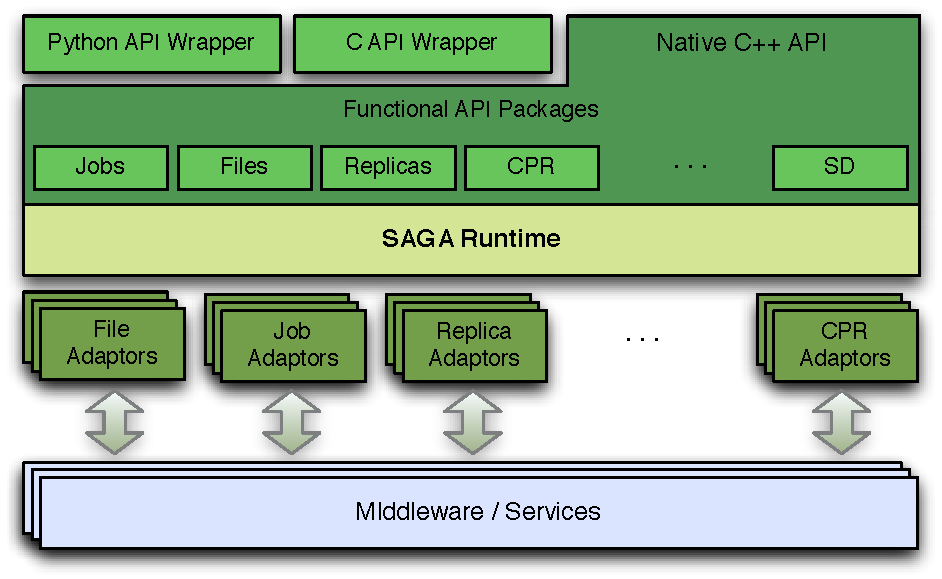
\includegraphics[scale=0.5]{saga-figure02.pdf}
 \caption{The SAGA runtime engine dynamically dispatches high level
          API calls to a variety of middlewares.}
 \label{fig:saga}
\end{figure}

Fig.~\ref{fig:saga} provides an overview of the SAGA programming
system's architecture.  The SAGA API covers job submission, file
access and transfer, as well as logical file management.  Additionally
there is support for Checkpoint and Recovery (CPR), Service Discovery
(SD), and other areas.  The API is implemented in C++ and Java, with
Python supported as a wrapper. \I{saga\_core} is the main library,
which provides dynamic support for run-time environment decision
making through loading relevant adaptors. We will not discuss SAGA
internals here; details can be found elsewhere~\cite{saga_url,Kaiser:2006qp}.


\subsection{Interfacing SAGA to Grids and Clouds}

SAGA was originally developed primarily for compute-intensive grids.
Ref~\cite{saga_ccgrid09} demonstrated that in spite of its original
design constraints, SAGA can be used to develop data-intensive
applications in diverse distributed environments, including clouds.
This is in part due to the fact that, at least on application level,
much of the ``distributed functionality'' required for data-intensive
applications remains the same.  How the respective functionality for
grid systems and for EC2 based cloud environments is provided in SAGA
is also documented in~\cite{saga_ccgrid09}.  Based on those
experiences, we added another backend to the set, which allows to
extend the range of backend architectures available to SAGA-C++ to
Sector-Sphere~\cite{sectorsphere09}.


\subsubsection{Sector-Sphere Adaptors: Design and Implementation}

Sector and Sphere is a cloud framework specifically designed for
writing applications able to utilize the stream processing paradigm.
Sector is a distributed file system that manages data across physical
compute nodes at the file level, and provides the infrastructure to
manipulate data in the cloud.  Sphere, on the other hand, provides the
framework to utilize the stream processing paradigm for processing the
data residing on Sector.  The Sphere system is composed of Sphere
Processing Engines (SPEs) running on the same physical nodes as the
Sector file system.

Applications that utilize the stream processing paradigm define a
single common function (aka kernel) that is applied to segments of a
given data set.  When the application invokes Sphere to process data
on Sector, the Sphere system retrieves the stream of data, segments
the data and assigns chunks of these segments to the available SPEs
for processing.

Sphere allows the user to encode the kernel function in a dynamically
linked library written against the Sphere APIs.  The SPEs apply this
user defined function to its assigned segments and write the
processing results back to files in Sector.  This stream of output
files can be retrieved by the user from Sector, after the processing
is complete. 

% \ssnote{Maybe add a different section here}
% \ssnote{Add another section here for experiments, or maybe later after
% MapReduce description} 

\paragraph{SAGA adaptor overhead:} \label{ssec:overhead}

We execute a simple experiment to measure the overhead introduced by
submitting Sphere jobs and Sector file operations through SAGA.  The
used sample Sphere kernel function accepts a buffer of text and
utilizes the Sphere framework to hash words into Sphere buckets, using
the first letter as the key. One Gigabyte of text data was uploaded to
the Sector file system for this test.  Furthermore, traces were
implemented in the adaptors to measure the exact time spent in SAGA
processing and translation before the raw Sphere APIs were called.  As
seen in Table ~\ref{tab:sphere_overhead}, the SAGA overhead is, if compared
to the overall execution time of the application, negligible.
This makes SAGA an excellent platform to compare Sphere with other distinct
programming models.
\miklosnote{Saurabh: Please check/update the description for the table.}

\begin{table}[h!]
  \footnotesize
  \begin{tabular}{cccc}
    \hline
    & Vanilla Sphere &  SAGA-Sphere & Adaptor \\
    &                &              & overhead \\
    \hline
    { {\bf Mean}} & 3.1858 & 4.1034 & 0.436 \\
    \hline 
    { {\bf Stdev}} & 0.5174 & 1.2464 & 0.0787 \\
    \hline \hline
  \end{tabular}
  \caption{Adaptor overhead measurements from processing 8GBs of data with 8
  SPEs running the \wc application on 8 physical nodes on Poseidon.
  All times are in minutes, aggregated from 10 runs.\uppp
  \label{tab:sphere_overhead}}
\end{table}


Thanks to the low overhead of developing SAGA adaptors, we were able
to implement the Sector file adaptor, and the Sphere job adaptor for
applications to utilize the stream processing paradigm through SAGA.
\F{Figure} and \F{Figure} give simple examples of how SAGA APIs
can be used to manipulate data in the Sector systems, and how jobs can
be submitted to the Sphere system to process this data.  The
enhancement of \sagamapreduce, along with the implementation of the
Sector/Sphere adaptors naturally gives us the opportunity to compare
and study these two distinct programming models.


\section{SAGA-based MapReduce}
\label{sec:mr}

 Given its relevance~\cite{saga_ccgrid09}, we choose the \smr
 implementation to compare both different backend systems (grids,
 clouds, clusters) and different programming models (master/slave,
 Sector-Sphere streams).  A simple \wc application on top of
 \smr has been used as a close-to-reality test case, and is
 described in Sec.~\ref{ssec:app}.

% After \sagamapreduce we have also developed real scientific
% applications using SAGA based implementations of patterns for
% data-intensive computing: multiple sequence alignment can be
% orchestrated using the SAGA-All-pairs implementation, and genome
% searching can be implemented using SAGA-MapReduce (see
% Ref.~\cite{saga_ccgrid09}).
% \upp

\subsection{\sagamapreduce Implementation}

\jhanote{Miklos to fix and update to reflect latest version of
  MapReduce}

Our implementation of \sagamapreduce interleaves the core \mr logic
with explicit instructions on where processes are to be scheduled.
The advantage of this approach is that our implementation is no longer
bound to run on a system providing the appropriate semantics
originally required by MapReduce, and is portable to a broader range
of generic systems as well.  The drawback is that it is more
complicated to extract performance, as some system level semantics has
to be recreated in application space (i.e., on SAGA or \smr) level.
% -- for there is a need to add system
% semantic capabilities at some level, and it is inherently slower --
% as it is difficult to reproduce system-specific optimizations to
% work generically.
The fact that the implementation is single-threaded proved to be the
primary current performance inhibitor.  However, none of these
complexities are exposed to the end-user, as they remain hidden within
the framework. 

% Also many of the complexities are due to the early-stages of SAGA
% and incomplete implementation of features, and not a fundamental
% limitation of the design or concept of the interface or programming
% models that it supports.  Future SAGA API packages will allow to
% alleviate some of these issues.

% The overall architecture of the SAGA-MapReduce implementation is
% shown in Fig.~\ref{saga-mapreduce_controlflow}. 
\smr exposes a simple interface which provides the complete
functionality needed by any MapReduce algorithm, while hiding the more
complex functionality, such as chunking of the input, sorting the
intermediate results, launching and coordinating the workers, etc. --
these are generically implemented by the framework.  The application
consists of two independent processes, a master and worker processes.
The master process is responsible for:

\begin{itemize}

 \item launching all workers for the map and reduce steps, as
 described in a configuration file provided by the user; and

 \item coordinating the workers, chunking of the data, assigning the
 input data to the workers of the map step, handling the intermediate
 data files produced by the map step, passing the location of the
 sorted output files to the workers of the reduce step.  

% \item re-launching single worker instances in case of failures, thus
% providing fail safety.
% \miklosnote{fail safety since it's not actually present.

\end{itemize}

The master process is readily available to the user and needs no
modification for different map and reduce functions to execute.  The
worker processes get assigned work either from the map or the reduce
step. The functionality for the different steps have to be provided by
the user, which means the user has to write two C++ functions
implementing the respective MapReduce kernels.

Both the master and the worker processes use the SAGA-API as an
abstract interface to the used infrastructure, making the application
portable between different architectures and systems.  The worker
processes are launched using the SAGA job package, allowing the jobs
to launch either locally, on globus/GRAM backends, on EC2 instances, through SSH
or on a Condor pool. The communication between the master and workers
is ensured by using the SAGA advert package, abstracting an
information database in a platform independent way, and the SAGA stream
package, abstracting streaming data access between network endpoints.
The master creates logical partitions of the data (referred to as chunking,
analogous to Google's MapReduce), so the data-set does not have to be split
and distributed manually.  The input data can be located on any file system
supported by SAGA, such as the local file system or a distributed file system
like HDFS or KFS \cite{KFS}.


\subsection{Enhancing SAGA-based Map-Reduce Performance}

The performance enhancements to the \sagamapreduce implementation as
discussed in~\cite{saga_ccgrid09} are based on two important changes:
(i) rearranging the shuffle phase, and (ii) using a serialized binary
format instead of plain text for intermediate data storage (also
available as an input and output format).  The first change means
that, instead of having the master merge and then sort the
intermediate data by key before doing the reduce phase, the workers
buffer key/value pairs from the map phase and store them in sorted
order on disk, doing an in-memory sort before writing. Also, since
intermediate key/value pairs from a map worker are already sorted, the
reduce workers need to only merge these pairs coming from different
map workers while applying the user-defined reduce function to the
merged intermediate key and value list.  The second enhancement
applies to the storage of the intermediate key/value pairs in a
so-called \emph{sequence file format}. This file format allows storing
of serialized key/value objects which can be read and merged much
faster in the reduce phase than text data, as there is no need for
costly parsing.  We used the Google Protocol Buffers library for
implementing serialization~\cite{protobuf}.  The processing of input
and output key/value pairs is further enhanced by minimizing
unnecessary memory I/O operations using a zero-copy scheme.


\subsection{\sagamapreduce Set-Up}

As with any application which concurrently spans multiple diverse
resources or infrastructures, the coordination between the different
application components becomes challenging.  The \smr implementation
uses the SAGA advert API for that task, and can thus limit the a-priory
information needed for bootstrapping the application: the compute
clients (workers) require (i) the contact address of the used advert
service instance, and (ii) a unique worker ID to register with in that
advert service, so that the master can start to assign work items.
Both information are provided by the master via command line
parameters to the worker, at startup time.

The master application requires the following additional information:
(i) a set of resources where the workers can execute, (ii) the
location of the input data, (iii) the target location for the output
data, and (iv) the contact point for the advert service for
coordination and communication.  

In a typical configuration, for example, three worker instances could
be started; the first could be started via GRAM and PBS on
qb.teragrid.org, the second on a pre-instantiated EC2 image
(instance-id \T{i-760c8c1f}), and the third on a dynamically deployed
EC2 instance (no instance id given).  Note that the startup times for
the individual workers may vary over several orders of magnitudes,
depending on the PBS queue waiting time and VM startup time.  The
MapReduce master will start to utilize workers as soon as they are
able to register themselves, so will not wait until all workers are
available.  That mechanism both minimizes time-to-solution, and
maximizes resilience against worker loss.
%
% The scheme \T{any} acts here as a placeholder for SAGA, so that the
% SAGA engine can choose an appropriate adaptor.  The master would
% access the file via the default local file adaptor.  The globus
% clients may use either the GridFTP or SSH adaptor for remote file
% success (but in our experimental setup would also succeed using the
% local file adaptor, as the Lustre FS is mounted on the cluster
% nodes), and the EC2 workers would use the ssh file adaptor for
% remote access.  Thus, the use of the placeholder scheme frees us
% from specifying and maintaining a concise list of remote data access
% mechanisms per worker.  Also, it facilitates additional resilience
% against service errors and changing configurations, as it leaves it
% up to the SAGA engine's adaptor selection mechanism to find a
% suitable access mechanism at runtime.  A parameter not shown in the
% above configuration example 
%
A simple parameter controls the number of workers created on each
compute node; as we will see by varying this parameter, the chances
are good that compute and communication times can be interleaved, and
that the overall system utilization can increase (especially in the
absence of precise knowledge of the execution system).
 

\section{Application Level Interoperability: Three-levels}
\label{sec:interop}

The motivation of ALI across multiple, heteregenous and distributed
resources follows from large-scale scientific applications, such as
the Earth Science Grid and LEAD. However for simplicity of treatment
and to focus on the levels of interoperability we will use a simple,
self-contained application, that has also become the {\it canonical}
\mr application-driver -- \wc.

\subsection{Application: \Wc}
\label{ssec:app}

We use our own implementations of the well known \wc application for
our experiments.  \Wc has a well understood runtime and scaling
behaviour, and thus serves us well for focusing the tests on the used
frameworks and middlewares.

The \mr based \wc implementation is described in~\cite{saga_ccgrid09}.
For the Sector-Sphere version of \wc, we implemented two kernel
functions. The first kernel function is responsible for hashing the
words in the data set into different hashing "buckets", depending on
the word's starting letter.  The standard C++ collate hashing function
was used for this purpose.  The second kernel function reads each hash
bucket, sorts the words in memory and outputs the final count value of
the words in the data set.  For example, a file containing the words
\T{('bread' 'bee' 'bee' 'honey')} would be hashed into buckets as
\T{('bread' 'bee' 'bee')} and \T{('honey')}.  The second kernel
function would read these intermediate bucket files, sort the words,
and produce the following result .  \T{(.bread 1., .bee 2., .honey
  1.)}.  The Sphere system is responsible for assigning files for
processing, synchronization, and writing output results back to
Sector.

\subsection{Interoperability Types}

Using the \wc application, we will demonstrate three types of
application level interoperability. We outline them here:

% different levels/types of interoperability.

\subsubsection{Type I: Application Interoperability via adaptors}
%
% Type I:  Application 
%              |
%           SAGA-MR
%              |
%           Adaptors
%      /     /   \      \
%    ... Clouds  Grids ...
%

As discussed, SAGA provides the ability to load a wide-range of
system-specifc adaptors dynamically. Thus a simple form of
interoperability, possibly specific to applications developed using
SAGA, is that an application can use any distributed systems without
changes to the application, thus experiencing cloud-cloud or
grid-cloud interoperability.  We refer to this as Type I
interoperabilty.

% interoperability quite trivially thanks to the dynamic loading of
% adaptors.  A

Thanks to the relative simplicity of developing SAGA adaptors, SAGA
has been successful interfaced to three cloud systems -- Amazon's EC2,
Eucalyptus~\cite{eucalyptus} (a local installation of Eucalyptus at
LSU) and Nimbus~\cite{nimbus}; and also to a multitude of grid based
environments, including TeraGrid, Loni and NGS.  SAGA based
applications are thus inherently able to utilize this form of ALI.

\subsubsection{Type II: Application Interoperability using programming
  models} % suited for different infrastructure}
%
% Type II:      Application 
%                    |
%          Instance-1 Instance-2
%            |            |
%         SAGA-Sphere SAGA-MapReduce
%            |            |
%       Sector-Sphere cluster/grids
%

Interoperabilty at a higher level than adaptors is both possible and
often desirable. An application can be considered interoperable if it
is able to switch between backend specific programming models.  We
will discuss an example where the \wc application is implemented so
that it can utilize either a Sector-Sphere framework via SAGA for the
OCC backend, or the \smr framework for generic grid and cloud
backends.


\subsubsection{Type III: Application Interoperability using different
  programming models for concurrent execution}
%
% Type III:   Application
%                 |
%     SAGA-Sphere / SAGA-MapReduce
%                 |
%   Sector-Sphere / cluster / grids / clouds
%

At another abstraction level, an application can also be considered
interoperable when it can \I{concurrently} execute multiple
programming model over multiple, diverse backends.  We demonstrate
that a \wc application uses Sector-Sphere and \smr to span multiple
backends.  The challenges of having different parts of an application
execute concurrently using different programming models is
conceptually different to loading different adaptors
concurrently. Thus we describe this as a separate type of
interoperability.

\subsection{Experimental Setup}

Simulations were performed on shared TeraGrid-LONI (Louisiana Optical
Network Initiative)~\cite{loni-url} resources running Globus and ssh;
on GumboGrid, a small cluster at LSU running Eucalyptus; on Amazon's
EC2; on a bare 50 node cluster of the Hungarian Academy of Sciences;
and on the OCC testbed~\cite{occ_testbed} running Sector-Sphere.  Jobs
are started via the respectively available middlewares, via SAGA's job
API.  Data exchange is either performed via streams, or via SAGA's
file transfer API which can dynamically switch between the various
available protocols.

For the could environments, we support the runtime configuration of VM
instances by staging a preparation script to the VM after its
creation, and executing it with root permissions.  In particular for
apt-get Linux distribution, the post-instantiation software deployment
is actually fairly painless, but naturally adds a significant amount
of time to the overall VM startup (which encourages the use of
preconfigured images).

For experiments in this paper, we prepared custom VM images with all
prerequisites pre-installed.  We utilize the preparation script solely
for some fine tuning of parameters: for example, we are able to deploy
custom saga.ini files, or ensure the finalization of service startups
before application deployment

Deploying \sagamapreduce framework and the \wc application on
different grids, clouds or clusters requires to adapt the configuration
to the specific environment.  For example, when running \sagamapreduce
on EC2, the master process resides on one VM, while workers reside on
different VMs.  Depending on the available adaptors, Master and Worker
can either perform local I/O on a global/distributed file system, or
remote I/O on a remote, non-shared file system.

It must be noted that we utilized different \smr versions for the
described experiments: the work described in this paper spans more
than 18 months, and the \smr implementation has simply evolved over
time.  As our primary goal is to dmeonstrate interoperability, and not
to document maximal performance, we consider those results valid
nonetheless.


\section{Experiments} 
\label{sec:exp}

\subsection{Type I ALI: Interoperability via Adaptors}

In an earlier paper (Ref~\cite{saga_ccgrid09}), we performed tests to
demonstrate how \sagamapreduce utilizes different infrastructures and
provides control over task-data placement; this led to insight into
performance on ``vanilla'' grids.  The primary aim of the work
presented here is to establish the fact that \sagamapreduce can
provide cloud-cloud interoperability and cloud-grid interoperability.
We performed the following experiments:

\begin{enumerate}

 \item We compare the performance of \sagamapreduce when exclusively
 running on a cloud platform to that when on grids. We vary the number
 of workers (1 to 10) and the data-set sizes varying from 10MB to 1GB.

 \item For clouds, we then vary the number of workers per VM, such
 that the ratio is 1:2 and 1:4, respectively.

 \item We then distribute the same number of workers across two
 different clouds - EC2 and Eucalyptus.

 \item Finally, for a single master, we distribute workers across
 grids (QueenBee on the TeraGrid) and clouds (EC2 and Eucalyptus) with
 one job per VM.

\end{enumerate}

It is worth reiterating, that although we have captured concrete
performance figures, it is not the aim of this work to analyze the
data and provide a performance model. In fact it is difficult to
understand performance implications, as a detailed analysis of the
data and understanding the performance will involve the generation of
``system probes'', as there are differences in the specific cloud
system implementation and deployment.  In a nutshell without adjusting
for different system implementations, it is difficult to rigorously
compare performance figures for different configurations on different
machines. At best we can currently derive trends and qualitative
information.  Any further analysis is considered out of scope for this
paper.

It takes SAGA about 45s to instantiate a VM on Eucalyptus and about
200s on average on EC2.  We find that the size of the image (say 5GB
versus 10GB) influences the time to instantiate an image, but is
within image-to-image instantiation time fluctuation.  Once
instantiated, it takes from 1-10s to assign a job to an existing VM on
Eucalyptus, or EC2.  The option to tie the VM lifetime to the
\T{saga::job\_service} object lifetime is a configurable option.  It
is also a matter of simple configuration to vary how many jobs (in
this case workers) are assigned to a single VM:  the default is 1
worker per VM.  The ability to vary this number is important -- as
details of actual VMs can differ as well as useful for our
experiments.


\subsubsection*{Results and Analysis}

The total time to solution ($T_s$) of a \sagamapreduce job can be
decomposed as the sum of three primary components -- $t_{pre},
t_{comp}$ and $t_{coord}$.  Here $t_{pre}$ is defined as
pre-processing time, which covers the time to chunk the data into
fixed size data units, to distribute them, and also to spawn the job.
$t_{pre}$ does not include the time required to start VM instances.
$t_{comp}$ is the time to actually compute the map and reduce function
on a given worker, whilst $t_{coord}$ is the time taken to assign the
payload to a worker, update records and to possibly move workers to a
destination resource; in general, $t_{coord}$ scales as the number of
workers increases.

Table~\ref{tab:1a} shows performance measurements for a variety of
worker placement configurations.  The master places the workers on
either clouds or on the TeraGrid (TG). The configurations -- separated
by horizontal lines, are classified as either all workers on the TG or
having all workers on EC2. For the latter, unless otherwise indicated
parenthesis, every worker is assigned to a unique VM. In the final set
of rows, the number in parenthesis indicates the number of VMs used.
Note that the spawning times depends on the number of VMs, even if it
does not include the VM startup times.  Table~\ref{tab:1b} shows data
from our interoperability tests.  The first set of data establishes
cloud-cloud interoperability. The second set (rows 5--11) shows
interoperability between grids-clouds (EC2).  The experimental
conditions and measurements are similar to Table 1.

\begin{table}[h!]
  \footnotesize
  \begin{tabular}{cccccc}
    \hline
    \multicolumn{2}{c}{\#workers}  &  Data size   &  $T_s$  & $T_{sp}$ & $T_s - T_{sp}$\\   
    TG &  AWS &   (MB)  & (sec) & (sec)  & (sec) \\
    \hline
  %  \textcolor{blue}{4} & - & 10  &  8.8 &  6.8 & 2.0 \\
    { {\bf 4}} & - & 10  &  8.8 &  6.8 & 2.0 \\
  %  \textcolor{blue}{6} & - & 10  &  12.4 &  10.2 & 2.2 \\
  %  10 & -  & 100 & 10.4 & 8.86 \\
  %  \textcolor{blue}{10} & - & 10  & 20.8 & 17.3 & 3.5 \\  
    \hline 
    - & 1 & 10 & 4.3 & 2.8 & 1.5 \\
    - & 2 & 10 & 7.8 & 5.3 & 2.5 \\ 
    - & 3 & 10 & 8.7 & 7.7 & 1.0 \\
    - & {\bf 4} & 10 & 13.0 & 10.3 & 2.7 \\
    - & 4 (1) & 10 & 11.3 & 8.6 & 2.7 \\
    - & 4 (2) & 10 & 11.6 & 9.5 & 2.1 \\
    \hline 
    -  & 2  & 100 & 7.9  & 5.3 & 2.6 \\
    -  & {\bf 4}  & 100 & 12.4 & 9.2 & 3.2\\
    -  & 10 & 100 & 29.0 & 25.1 & 3.9 \\
    \hline
    - & {\bf 4 (1)} & 100 & 16.2 & 8.7 & 7.5 \\ 
    - & {\bf 4 (2)} & 100 & 12.3 & 8.5 & 3.8 \\
    - & 6 (3) & 100 & 18.7 & 13.5 & 5.2\\
    - & 8 (1) & 100 & 31.1 & 18.3 & 12.8 \\
    - & 8 (2) & 100 & 27.9 & 19.8 & 8.1\\
    - & 8 (4) & 100 & 27.4 & 19.9 & 7.5\\
    \hline \hline
  \end{tabular}
  \caption{Performance data for different configurations of worker
  placements.\uppp
  \label{tab:1a}}
\end{table}

We find that in our experiments $t_{comp}$ is typically greater than
$t_{coord}$, but when the number of workers gets large, and/or the
computational load per worker small, $t_{coord}$ can dominate
(internet-scale communication) and increase faster than $t_{comp}$
decreases, thus overall $T_s$ can increase for the same data-set size,
even though the number of independent workers increases.  The number
of workers associated with a VM also influences the performance, as
well as the time to spawn; for example -- as shown by the three lower
boldface entries in Table 1, although 4 identical workers are used
depending upon the number of VMs used, $T_c$ (defined as $T_S -
T_{spawn} $) can be different.  In this case, when 4 workers are
spread across 4 VMs (i.e. default case), $T_c$ is lowest, even though
$T_{spawn}$ is the highest; $T_c$ is highest when all four are
clustered onto 1 VM. When exactly the same experiment is performed
using data-set of size 10MB, it is interesting to observe that $T_c$
is the same for 4 workers distributed over 1 VM as it is for 4 VMs,
whilst when the performance for the case when  4 workers are
spread-over 2 VMs out-perform both (2.1s).

\begin{table}[h!]
  \footnotesize
  \begin{tabular}{ccccccc}
    \hline
    \multicolumn{3}{c}{\# workers}  &  Size   &  $T_s$  & $T_{sp}$ & $T_s - T_{sp}$\\   
    TG &  AWS & Eucal. &  (MB)  & (sec) & (sec) & (sec) \\
    \hline
    - & 1 & 1 & 10   & 5.3 & 3.8 & 1.5\\
    - & 2 & 2 & 10   & 10.7 & 8.8 & 1.9 \\
    - & 1 & 1 & 100  & 6.7 & 3.8 & 2.9\\
    - & 2 & 2 & 100  & 10.3 & 7.3 & 3.0\\
    \hline 
    1 & - & 1 & 10   & 4.7 & 3.3 & 1.4\\
    1 & - & 1 & 100  & 6.4 & 3.4 & 3.0\\
    \hline 
    {\bf 2} &   {\bf 2} & - & 10 & 7.4 & 5.9 & 1.5 \\
    3 & 3 & - & 10 & 11.6 & 10.3 & 1.6 \\
    4 & 4 & - & 10 & 13.7 & 11.6 & 2.1 \\
    5 & 5 & - & 10 & 33.2 & 29.4 & 3.8 \\ 
  %\textcolor{blue}{5} & \textcolor{blue}{5} & - & 10 & 33.2 & 29.4 & 3.8 \\ 
    10 & 10 & - & 10 & 32.2 & 28.8 & 2.4 \\
    \hline
     \hline 
  %   1 & 1 & - & 100 & 5.4 & 3.1 & 2.3\\
  %   3 & 3 & - & 100 & 11.1 & 8.7 & 2.4 \\
  \end{tabular}
  \caption{Performance data for different configurations of worker
  placements on TG, Eucalyptus-Cloud and EC2. \uppp
  \label{tab:1b}}
\end{table}

Table 2 shows performance figures when equal number of workers are
spread across two different systems; for the first set of rows,
workers are distributed on EC2 and Eucalyptus. For the next set of
rows, workers are distributed over the TG and Eucalyptus, and in the
final set of rows, workers are distributed between the TG and EC2.
Given the ability to distribute at will, we compare performance for
the following scenarios: (i) when 4 workers are distributed equally
(i.e., 2 each) across a TG machine and on EC2 (1.5s), with the
scenarios when, (ii) all 4 workers are either exclusively on EC2
(2.7s), (iii) or all workers are on the TG machine (2.0s) (see Table
1, boldface entries on the first and fifth line). It is {\it
  interesting} that in this case $T_c$ is lower in the distributed
case than when all workers are executed locally on either EC2 or TG;
we urge that not too much be read into this, as it is just a
coincidence that a {\it sweet spot} was found where on EC2, 4 workers
had a large spawning overhead compared to spawning 2 workers, and an
increase was in place for 2 workers on the TG. Also it is worth
reiterating that for the same configuration there are
experiment-to-experiment fluctuations (typically less than 1s).  The
ability to enhance performance by distributed (heterogeneous)
work-loads across different systems remains a distinct possibility,
however, we believe more systematic studies are required.
% \jhanote{Needs major addition and rewrite. Saurabh and Miklos take a
%   first pass please at adding}

% \jhanote{Enhanced SAGA-MR Performance versus Early-version of SAGA-MR}
%\jhanote{Miklos: You have the data for this in the ``\WC
%  Measurement'' tab of
%  \url{http://spreadsheets.google.com/ccc?key=0AvHZsmPSSmBmdHVUMWFuWEpQdFQyak5GeHhQRVJrMlE&hl=en}
%  Please plot and Explain. Related to the earlier sub-section
%  (``Enhancing SAGA-based MapReduce performance) }

% \miklosnote{Shantenu: Please correct figure's placement as suitable.}
% \jhanote{For the meantime at least, I think this is OK. But we need to 
%   describe (in the caption as well) which resources these comparisons were made
%   and what the configuration was}

The original \sagamapreduce version (as used for the experiments
presented above) physically chunked the input data files.  Our evolved
version, however, creates logical chunks (i.e., no file
writing takes place).  It is thus fair to compare their
time-to-solution performance by subtracting the chunking time from the
early-version's job completion time.  Fig.~\ref{fig:sagamr_comparison}
shows the thus corrected performance data for the early-version and
enhanced version of \sagamapreduce.  8 workers were spawned via the
SAGA SSH adaptor on 8 physical machines,  data were exchanged through
a shared NFS file system.  The figure shows that the \sagamapreduce
enhancements make a difference for larger data sets.  This can be
attributed to the fact that the more efficient shuffle phase
implementation, which reduces disk I/O and CPU usage in the reduce
phase by doing only a merge, outperforms the old implementation, which
performed a merge-sort of all the intermediate output files.

\begin{figure}[htb!]
 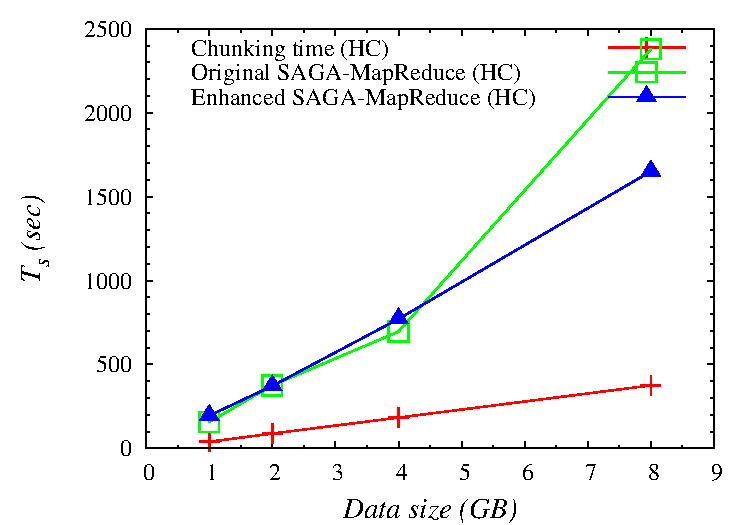
\includegraphics[width=0.5\textwidth]{figures/sagamr_comparison.pdf}
 \caption{
   Comparison of enhanced SAGA-MR performance versus
   early-version of SAGA-MR on the ILAB cluster using 8 workers running on 8
   physical machines. Jobs were launched via SSH and used NFS for file
   operations.
   \label{fig:sagamr_comparison}
   }
\end{figure}


\subsection{Type II ALI: Application Performance Using SAGA-based
Sphere and MapReduce}

\subsubsection{Experiment I -- Varying chunk sizes} 

For the Sector-Sphere based \wc, Sector maintains and tracks
data in the cloud at the file level. There is no support in Sphere to
control the chunk sizes of files assigned to the Sphere processing
engines. Therefore, to experiment with different chunk sizes, the
files were split manually into smaller chunks before the \wc
application was launched. In this set of experiments, we vary the
chunk size from 16 MB to 256 MB, while keeping the number of SPEs
constant to 8, and the data size constant to 4 GB. Each SPE is running
on a separate physical node in the cluster. These results are
presented in Fig.~\ref{fig:sphere_mr_chunksize}.
As evident from the results we collected, a
correlation exists between the chunk sizes and performance of Sphere.
As the chunk sizes increase, the performance deteriorates. Also, we
observe a major decline in performance right after the 64 MB data
point. 

\begin{figure}[htb!]
 \upp \upp
 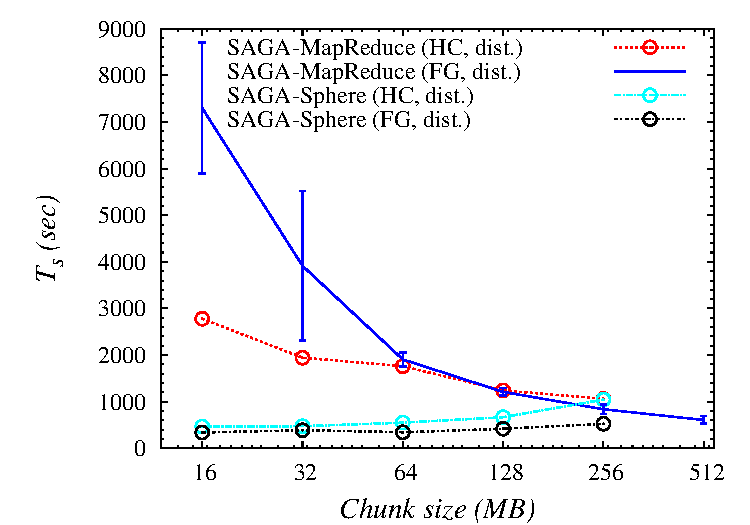
\includegraphics[width=0.5\textwidth]{figures/sphere_mr_varying_chunksize.pdf}
 \upp \upp
 \caption{
   Comparison of enhanced SAGA-MR performance versus
   SAGA-Sphere performance when varying chunk size while keeping the amount
   of processed data constant at 4GBs. Data and computation were
   distributed for these experiments.
   \label{fig:sphere_mr_chunksize}
   }
\end{figure}

We performed the same set of experiments with SAGA-MapReduce based
\wc and observe a completely different trend with respect to
chunk size and performance. We use a local file system accessible
through NFS for all the 8 workers and set the number of reduce tasks
to 8.  In case of SAGA-MapReduce performance increases with larger
chunk sizes, outperforming Sphere at the 256 MB data point. As it can
be seen in \F{Fig.xx} this can be attributed to the fact that
$t_{coord}$ dominates total time-to-solution for smaller chunk sizes.
The larger the chunk size the smaller the number of map tasks
launched, hence $t_{coord}$ decreases with increasing chunk size.


\subsubsection{Experiment II -- Varying Workers}

\begin{figure}[htb!]
 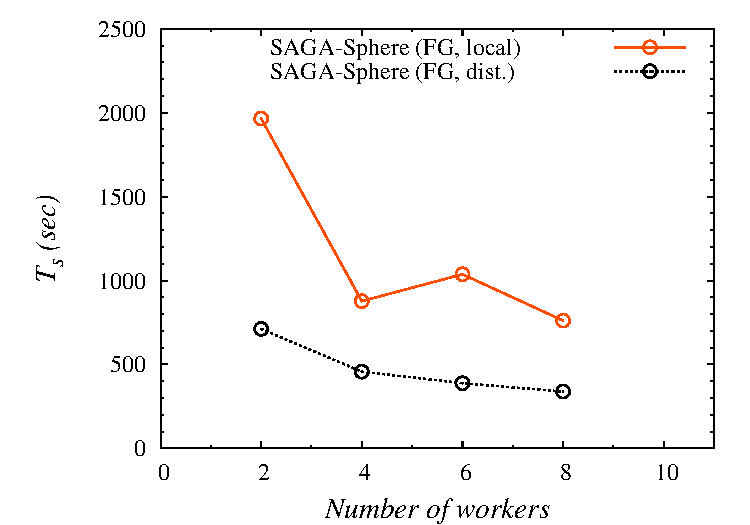
\includegraphics[width=0.5\textwidth]{figures/sphere_varying_workers.pdf}
 \caption{
   Comparison of SAGA-Sphere performance when varying the number of workers
   between 2 and 10 in two configurations: (1) local data and computation
   and (2) distributed data and computation.
   \label{fig:sphere_varying_workers}
   }
\end{figure}

We perform two sets of experiments with SAGA-Sphere running the same
\wc application.  We keep the chunk size constant at 64 MB, the
data size fixed at 4GB (as previously) but vary the number of workers
in two configurations. In the first configuration, we use Sphere on a
local data and local compute configuration. In the second
configuration, we observe how the solution scales to a distributed
data and distributed compute configuration. These results are
illustrated in Fig.~\ref{fig:sphere_varying_workers}.  For the local-local
configuration, we launch Sector and Sphere on a single physical node.
For the distribute-distribute configuration, we launch Sector and
Sphere on one physical node per SPE.  We observe the maximum peak
performance at 6 distributed workers. Sector can maintain file
replicas to achieve optimal data distribution between SPEs and
minimize synchronization overhead. For the purpose of our experiments,
we limited Sector to not create any replicas.

We perform similar measurements via \sagamapreduce: while keeping the
chunk size constant at 64MB and the data size at 4GB, we note the
time-to-solution of the \wc application in the two
configurations described for SAGA-Sphere above.  For the
distribute-distribute configuration we used HDFS as the distributed
file system and launched jobs using the SAGA SSH job adaptor.
Similarly to the varying chunk size experiments, we set the number of
reduce tasks to 8.  \miklosnote{Will describe local-local
configuration here.}

SAGA gives us the opportunity to experiment with different programming models very easily. 
As evident from the data plots in Figure xx and Figure yy, certain behavioral 
trends for SAGA-Sphere and SAGA-MapReduce emerge.  In Experiment 1, where we keep the 
number of workers constant and vary the chunk sizes, the trends between 
SAGA-MapReduce and Sphere are inversed: the Sphere performance deteriorates with 
increasing chunk sizes, while the performance of SAGA-MapReduce increases. This behavior
suggests that SAGA-MapReduce's synchronization overhead to manage smaller 
chunk sizes compared to the speed up achieved through parallelism is much higher. 
In the case of the \wc application, SAGA-MapReduce suggests to be more 
suitable for coarse grained computations. SAGA-Sphere, on the other hand, yields 
better performance from smaller chunks sizes (a larger amount of files) making it 
suitable for finer grained computations with better data distribution.

In Experiment 2, where we keep the chunk size to a constant of 64 MB, SAGA-Sphere 
exhibits a trend where adding more SPEs has a positive impact on performance. However, 
at the 8 SPEs and 10 SPEs data points, we see a decline in performance, possibly 
due to high synchronization costs between the workers. What is interesting to 
notice are the two data points - 8 SPEs @ 64 MB chunk size in Figure yy 
and 8 SPEs @ 16 MB chunk size in Figure xx. Reducing the chunk size by 75\%, 
thereby providing better data distribution with a larger number of files, we 
see almost a 65\% increase in performance. This further confirms our 
supposition that good data distribution had a major impact on Sphere's performance for
the \wc application. We do not claim that fine grained computation 
granularity is a concrete determinant of SAGA-Sphere's performance in a 
general case, but a noticeable aspect that emerges through its comparison with SAGA-MapReduce. 


\subsection{Type III ALI: Interoperability Concurrency}

We discuss the third type of interoperability in this section,
where SAGA-MapReduce and SAGA-Sphere are used in conjunction 
to solve the \wc problem. We first use the 'netperf' 
utility to measure the throughput from the client host to 
the SAGA-MapReduce master node and SAGA-Sphere master node. 
In our case, the throughput measured to the two nodes was 
approximately equal (935 MB/s to SAGA-Sphere and 925 MB/s to SAGA-MapReduce). 
Based on these metrics, we split the 4.0 GB data set 
into two equal 2.0 GB parts. This is to ensure that the data 
transfer time to both masters is approximately the same. We 
configured both systems to utilize 4 workers each 
and 64 MB chunk sizes. The data transfer time to the Sector 
cloud took a total of 97.8 seconds and 10.4 seconds to the 
SAGA-MapReduce master node. The longer transfer time to Sector 
can be credited to the overhead incurred from registering 
the files in Sector. The data transfer was done sequentially. 

We found that SAGA-Sphere took a total of 441.3 seconds to 
process the 2.0 GB data, while SAGA-MapReduce took a total of 
769 seconds. Aggregating the output results from the two systems 
took a negligible amount of time (only 0.9 seconds). The data was 
already sorted and hence could be merged in O(n) complexity. 
The above simple experiment of combining two varied programming 
models for solving a common problem paves the way to further 
investigation into smarter data and compute placement techniques. 
The total time taken to execute the \wc application in this 
case was approximately 877.9 seconds. It is interesting to 
note that this performance measure lies between 1329.96 seconds 
for 8 SPEs and 716 seconds for 8 SAGA-MapReduce workers at 
a 64 MB chunk size. 



\section{Discussion \& Conclusions}
\label{sec:discuss}

\jhanote{Recap three levels of Application Level Interoperability}

At the lowest level, \sagamapreduce demonstrates how to decouple the
development of applications from the deployment and details of the
run-time environment (Type I ALI).  It is critical to reiterate that
using this approach applications remain insulated from any underlying
changes in the infrastructure -- not just grids and different
middleware layers, but also different systems with very different
semantics and characteristics, whilst being exposed to the important
distributed functionality.  MapReduce has trivial data-parallelism, so
in the near future we plan to develop applications with non-trivial
data-access, transfer and scheduling characteristics and requirements,
and deploy different parts on different underlying infrastructure
guided by optimal performance.

With our two implementations of the same application framework, the
SAGA based Sector-Sphere framework, and the \smr implementation, we
demonstrated the Type II ALI: applications can seemlessly switch
between backends by switching frameworks.  Finally, by concurrently
using Sector-Sphere \mr and \smr, we demonstrated Type III ALI,
allowing the application to span a wide variety of backends
concurrently, and efficiently.

{\it Programming Models for Clouds: } Ref~\cite{jha_ccpe09} introduced
the notion of {\it affinity} for clouds to capture the idea of
relative data-compute placement and locality; it is imperative that
any programming model/system be cognizant of the notion of
affinity. We have implemented the first steps in a PM which provides
easy control over relative data-compute placement; a possible next
step would be to extend SAGA to directly support affinity (data-data,
data-compute).  There exist other emerging programming systems like
Dryad, Sawzall and Pig, which could be used in principle to support
the notion of affinity as well as develop/use MapReduce.  But it is
important to distinguish the infrastructure independence of
\sagamapreduce with the reliance of Google's
MapReduce~\cite{mapreduce-paper} on a number of capabilities of the
underlying system -- mostly related to file operations, but including
system features related to process/data allocation.

We will generalize our approach to most efficiently execute it by
taking into consideration the data-locality, as well as the access
patterns of the execution steps required to complete the work flow.
This analysis is done through developing performance models of
transferring data between frameworks, as well as the distribution of
the computing resources in the environment. Based on this analysis,
the data is placed efficiently, and a subset of nodes and frameworks
maybe chosen to perform the necessary computations. The shuffled data
is also cached for future computations.  We have embarked on the
creation of components that facilitate flexibility in data placement
relative to the computational resource -- that is either data can be
transferred intelligently to match computational workloads or
computational workloads can be placed to match (prevent) data
requirements~\cite{???}. More generically, it is worth mentioning that
these approaches can be extend to support certain kinds of {\it
affinities}.

\amnote{someone needs to check the paragraph above. Sounds like a lot
of handwaving ;-) What is the citation supposed to be?}


% A feature worth noting in MapReduce is that the ultimate dataset is
% not on one machine, it is partitioned on multiple machines
% distributed.

% Google use their distributed file system (Google File System) to keep
% track of where each file is located.  Additionally, they coordinate
% this effort with BigTable.

% {\it Simplicity versus Completeness:} There exist both technical
% reasons and social engineering problems responsible for low uptake of
% grids. One universally accepted reason is the complexity of grid
% systems -- the interface, software stack and underlying complexity of
% deploying distributed application. But this is also a consequence of
% the fact that grid interfaces tend to be ``complete'' or very close
% thereof.  % For example, while certainly not true of all cases, consider
% % the following numbers, which we believe represent the above points
% % well: globus 4.2 provides, in its Java version,
% % approximately 2,000 distinct method calls.  The complete SAGA Core
% % API~\cite{saga-core} provides roughly 200 distinct method calls.
% % The
% % SOAP rendering of the Amazon EC2 cloud interface provides,
% % approximately 30 method calls (and similar for other Amazon cloud
% % interfaces, such as Eucalyptus~\cite{eucalyptus}).
% The number of
% calls provided by these interfaces is no guarantee of simplicity of
% use, but is a strong indicator of the extent of system semantics
% exposed.  But to a first approximation, (simplicity of) interface
% determines the programming models that can be supported. Thus there is
% the classical trade-off between simplicity and completeness.

%\section{Conclusion and Some Future Directions}

% EC2 and Eucalyptus although distinct systems
% have similar interfaces; we will work towards developing SAGA based
% applications that can use very different infrastructures, e.g.,
% Google's AppEngine, such that \sagamapreduce uses Google's cloud
% infrastructure.

% Finally, it is worth mentioning that computing in the clouds for
% this project cost us upwards of \$300 to perform these experiments
% on EC2.

%   somewhat similar; a very different beast is Google's AppEngine.  We
%   will in the near future be working towards providing \sagamapreduce
%   via Google's AppEngine

% {Mention that Amazon and Eucalyptus although distinct are
%   somewhat similar; a very different beast is Google's AppEngine.  We
%   will in the near future be working towards providing \sagamapreduce
%   via Google's AppEngine}


% Patterns capture a dominant and recurring computational mode; by
% providing explicit support for such patterns, end-users and domain
% scientists can reformulate their scientific problems/applications so
% as to use these patterns.  This provides further motivation for
% abstractions at multiple-levels.


%\section{Acknowledgments}
\footnotesize{ {\noindent \bf Acknowledgments: }SJ acknowledges UK EPSRC grant
  number GR/D0766171/1 for supporting SAGA and the e-Science
  Institute, Edinburgh for the research theme, ``Distributed
  Programming Abstractions''.  SJ also acknowledges financial support
  from NSF-Cybertools and NIH-INBRE Grants, while ME acknowledges support
  from the grant OTKA NK 72845.  We also acknowledge
  internal resources of the Center for Computation \& Technology (CCT)
  at LSU and computer resources provided by LONI/TeraGrid for
  QueenBee.  We thank Chris Miceli, Michael Miceli, Katerina Stamou \&
  Hartmut Kaiser for their collaborative efforts on early parts of
  this work. We thank Mario Antonioletti and Neil Chue Hong for
  supporting this work through GSoC-2009 (OMII-UK Mentor
  Organization).}

\bibliographystyle{plain}
\bibliography{saga_data_intensive}

\end{document}

% This work would not have been possible without the efforts and
% support of other members of the SAGA team.  In particular,
% \sagamapreduce was originally written by Chris and Michael Miceli,
% as part of a Google Summer of Code Project, with assistance from
% Hartmut Kaiser. We also thank Hartmut for great support during the
% testing and deployment phases of this project. We are greatful to
% Dmitrii Zagorodnov (UCSB) and Archit Kulshrestha (CyD group, CCT)
% for the support in deployment with Eucalyptus.  KS would like to
% acknowledge the LSU Networking Infrastructure \& Research IT
% Enablement team for their help and support.
